\documentclass[../../compsys.tex]{subfiles}
\begin{document}
\raggedbottom
\chapter{L14 — Transport Layer and TCP}
\vfill
\raggedbottom

\section{Introduction to the Transport Layer}
\textit{Understanding the role and responsibilities of the transport layer in network communication.}

Throughout this semester, we have focused on the application layer, examining how processes interact through system calls and how applications like web clients, servers, and DNS operate. Today, we explore what happens beneath the application layer when processes make network system calls.

\subsection{Protocol Stack and Data Structures}
\textit{Understanding how data is transformed as it moves through network layers.}

The Internet uses a layered architecture where each layer adds header information:

\begin{enumerate}
  \item \textbf{Application Layer} — Creates \textbf{messages} for inter-process communication
  \item \textbf{Transport Layer} — Adds transport headers, creating:
  \begin{itemize}
    \item[-] \textbf{UDP datagrams} (User Datagram Protocol)
    \item[-] \textbf{TCP segments} (Transmission Control Protocol)
  \end{itemize}
  \item \textbf{Network Layer} — Adds IP headers, creating \textbf{IP packets}
\end{enumerate}

\begin{center}
  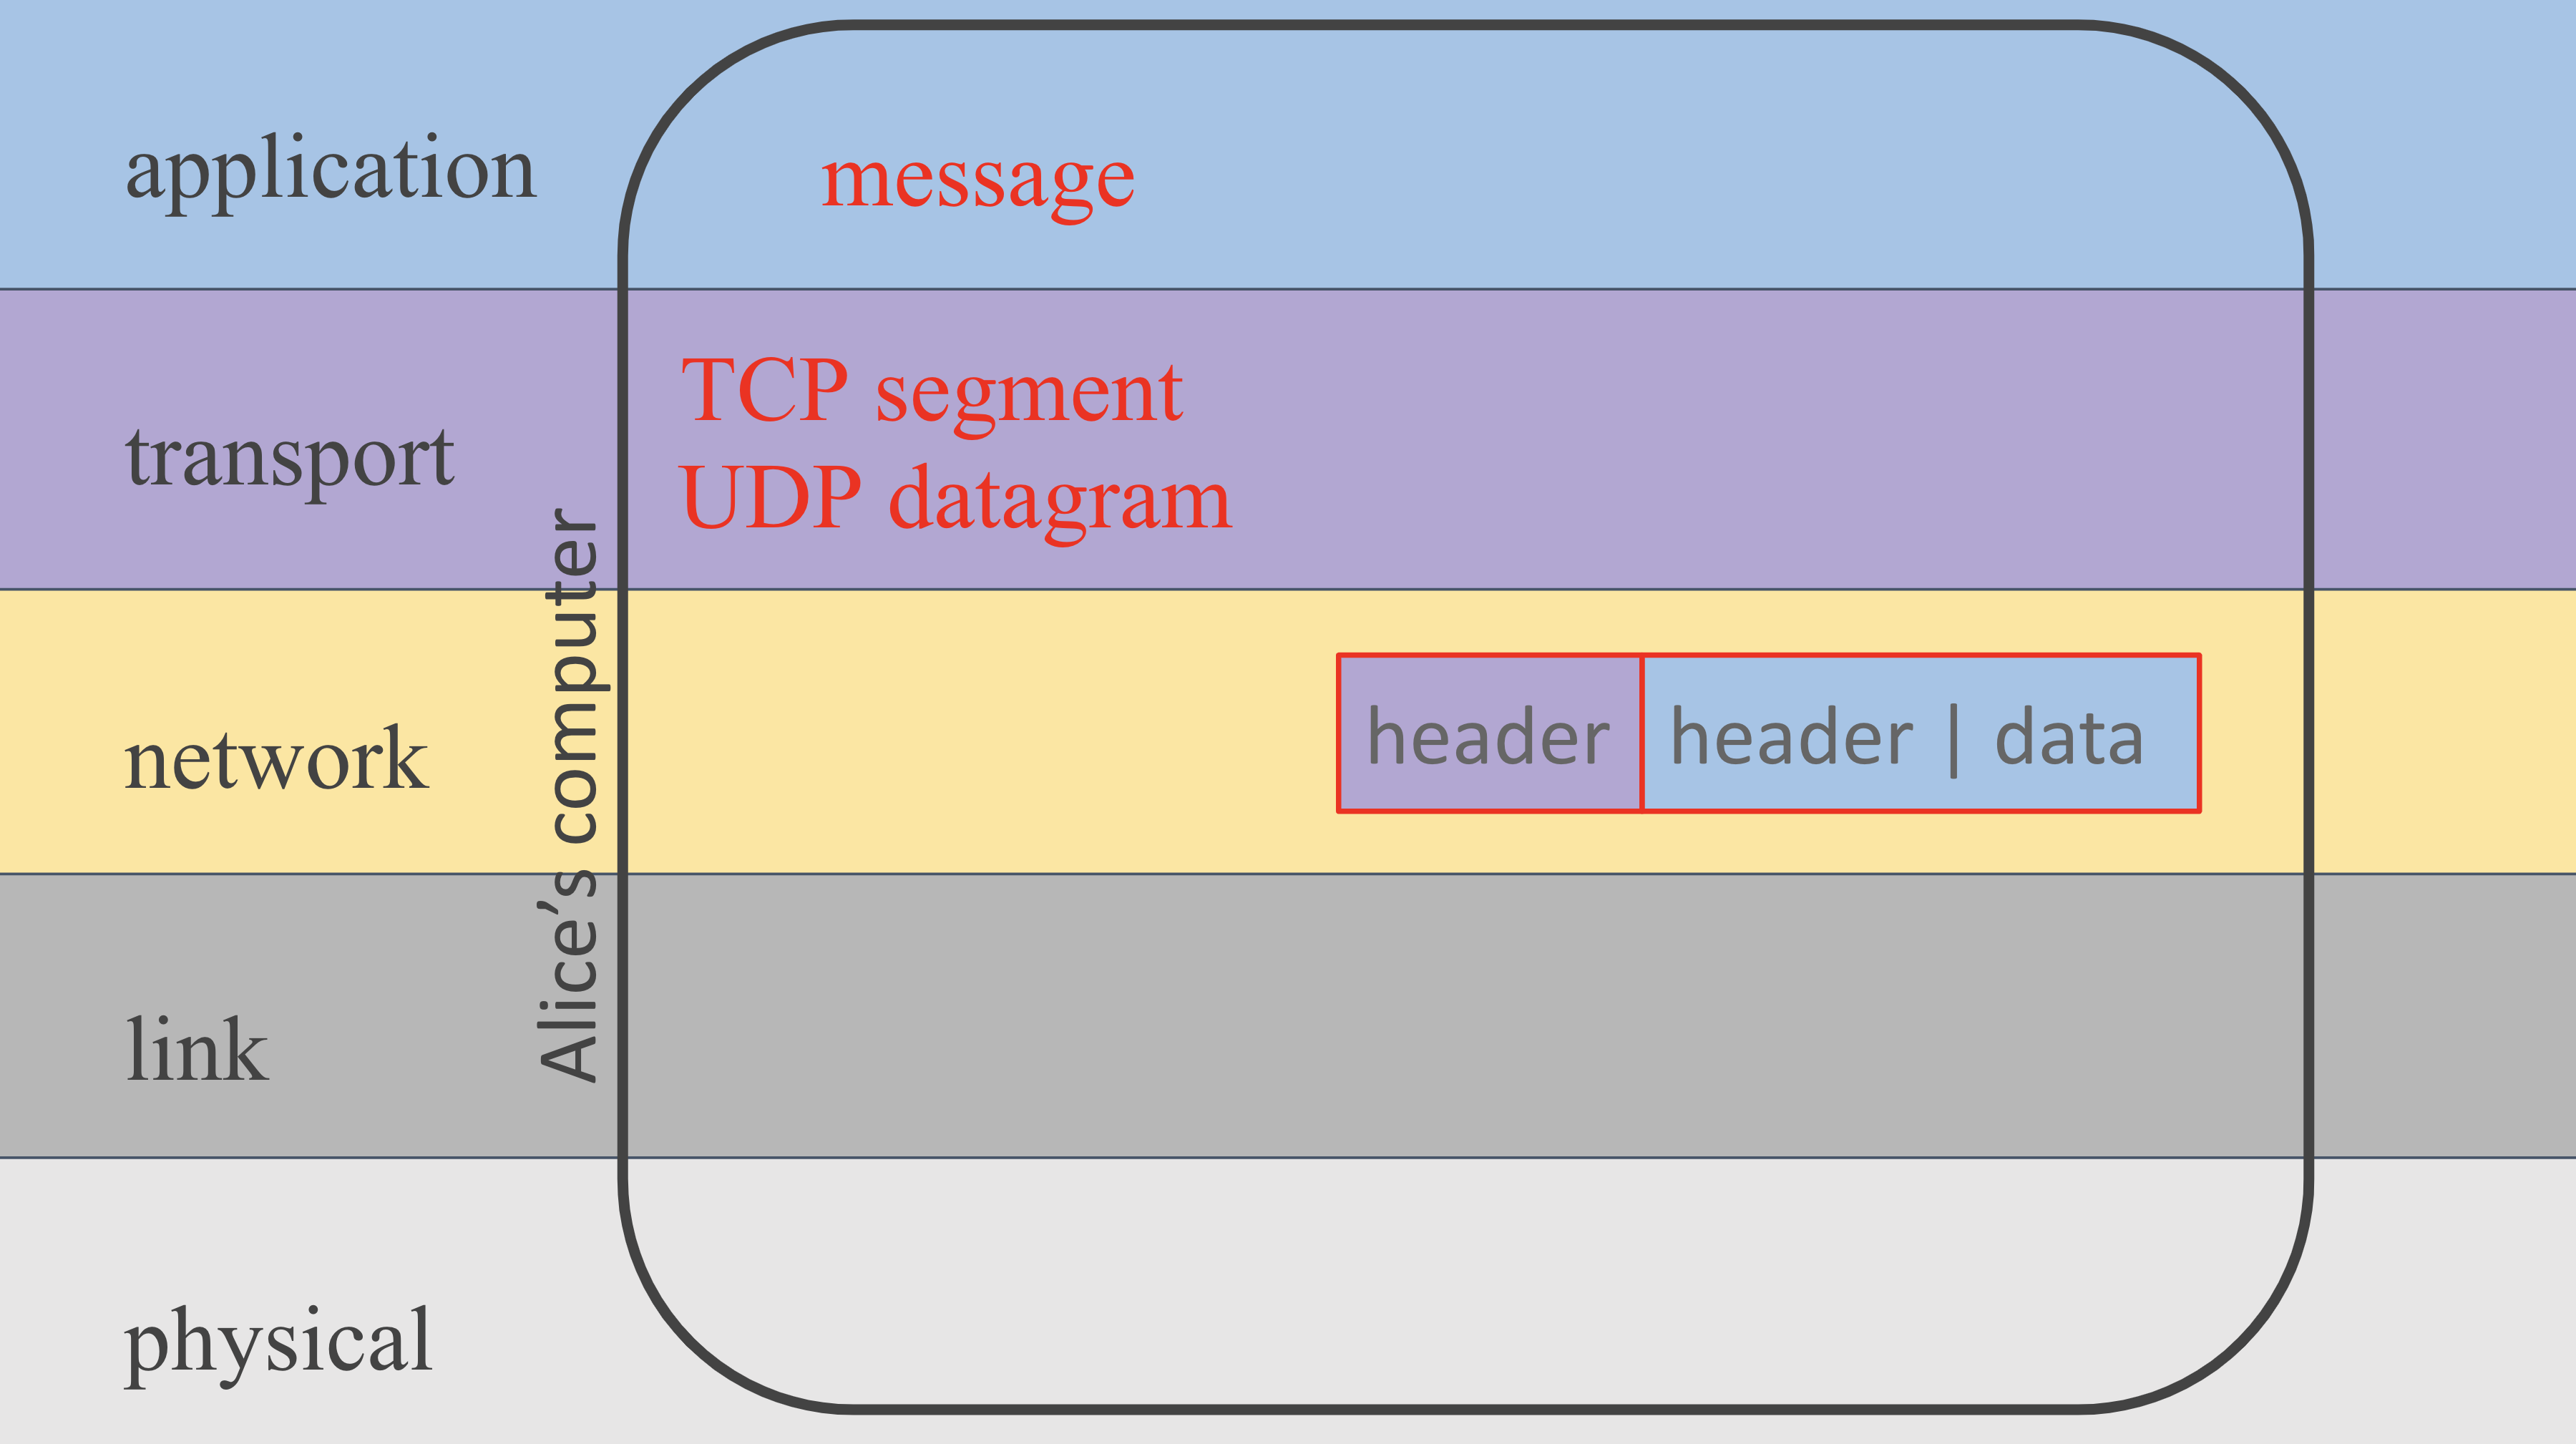
\includegraphics[width=0.5\textwidth]{images/layers.png}
\end{center}

The transport layer provides essential services enabling reliable process-to-process communication over an unreliable network infrastructure.

\section{User Datagram Protocol (UDP)}
\textit{A minimal transport protocol providing basic services with low overhead.}

UDP adds minimal functionality to the network layer, making it suitable for applications requiring low overhead that can tolerate data loss.

\subsection{UDP Services and Communication}
\textit{Core functions and operation of UDP.}

UDP provides three fundamental services:

\subsubsection{Multiplexing and Demultiplexing}
\begin{itemize}
  \item[-] \textbf{Multiplexing} — Handles messages from multiple application processes, encapsulating each in UDP datagrams
  \item[-] \textbf{Demultiplexing} — Uses port numbers to deliver incoming datagrams to the correct application process
  \item[-] Enables multiple applications to share network resources efficiently
\end{itemize}

\subsubsection{Basic Error Detection}
\begin{itemize}
  \item[-] \textbf{Checksum computation} — Sender computes checksum from header and data
  \item[-] \textbf{Integrity verification} — Receiver recomputes and compares checksums
  \item[-] \textbf{Corruption handling} — Corrupted datagrams are discarded
\end{itemize}

The checksum uses one's complement arithmetic on 16-bit words, providing simple but effective error detection for most transmission errors.

\subsection{UDP Communication Process}
\textit{Step-by-step UDP communication between client and server.}

\begin{center}
  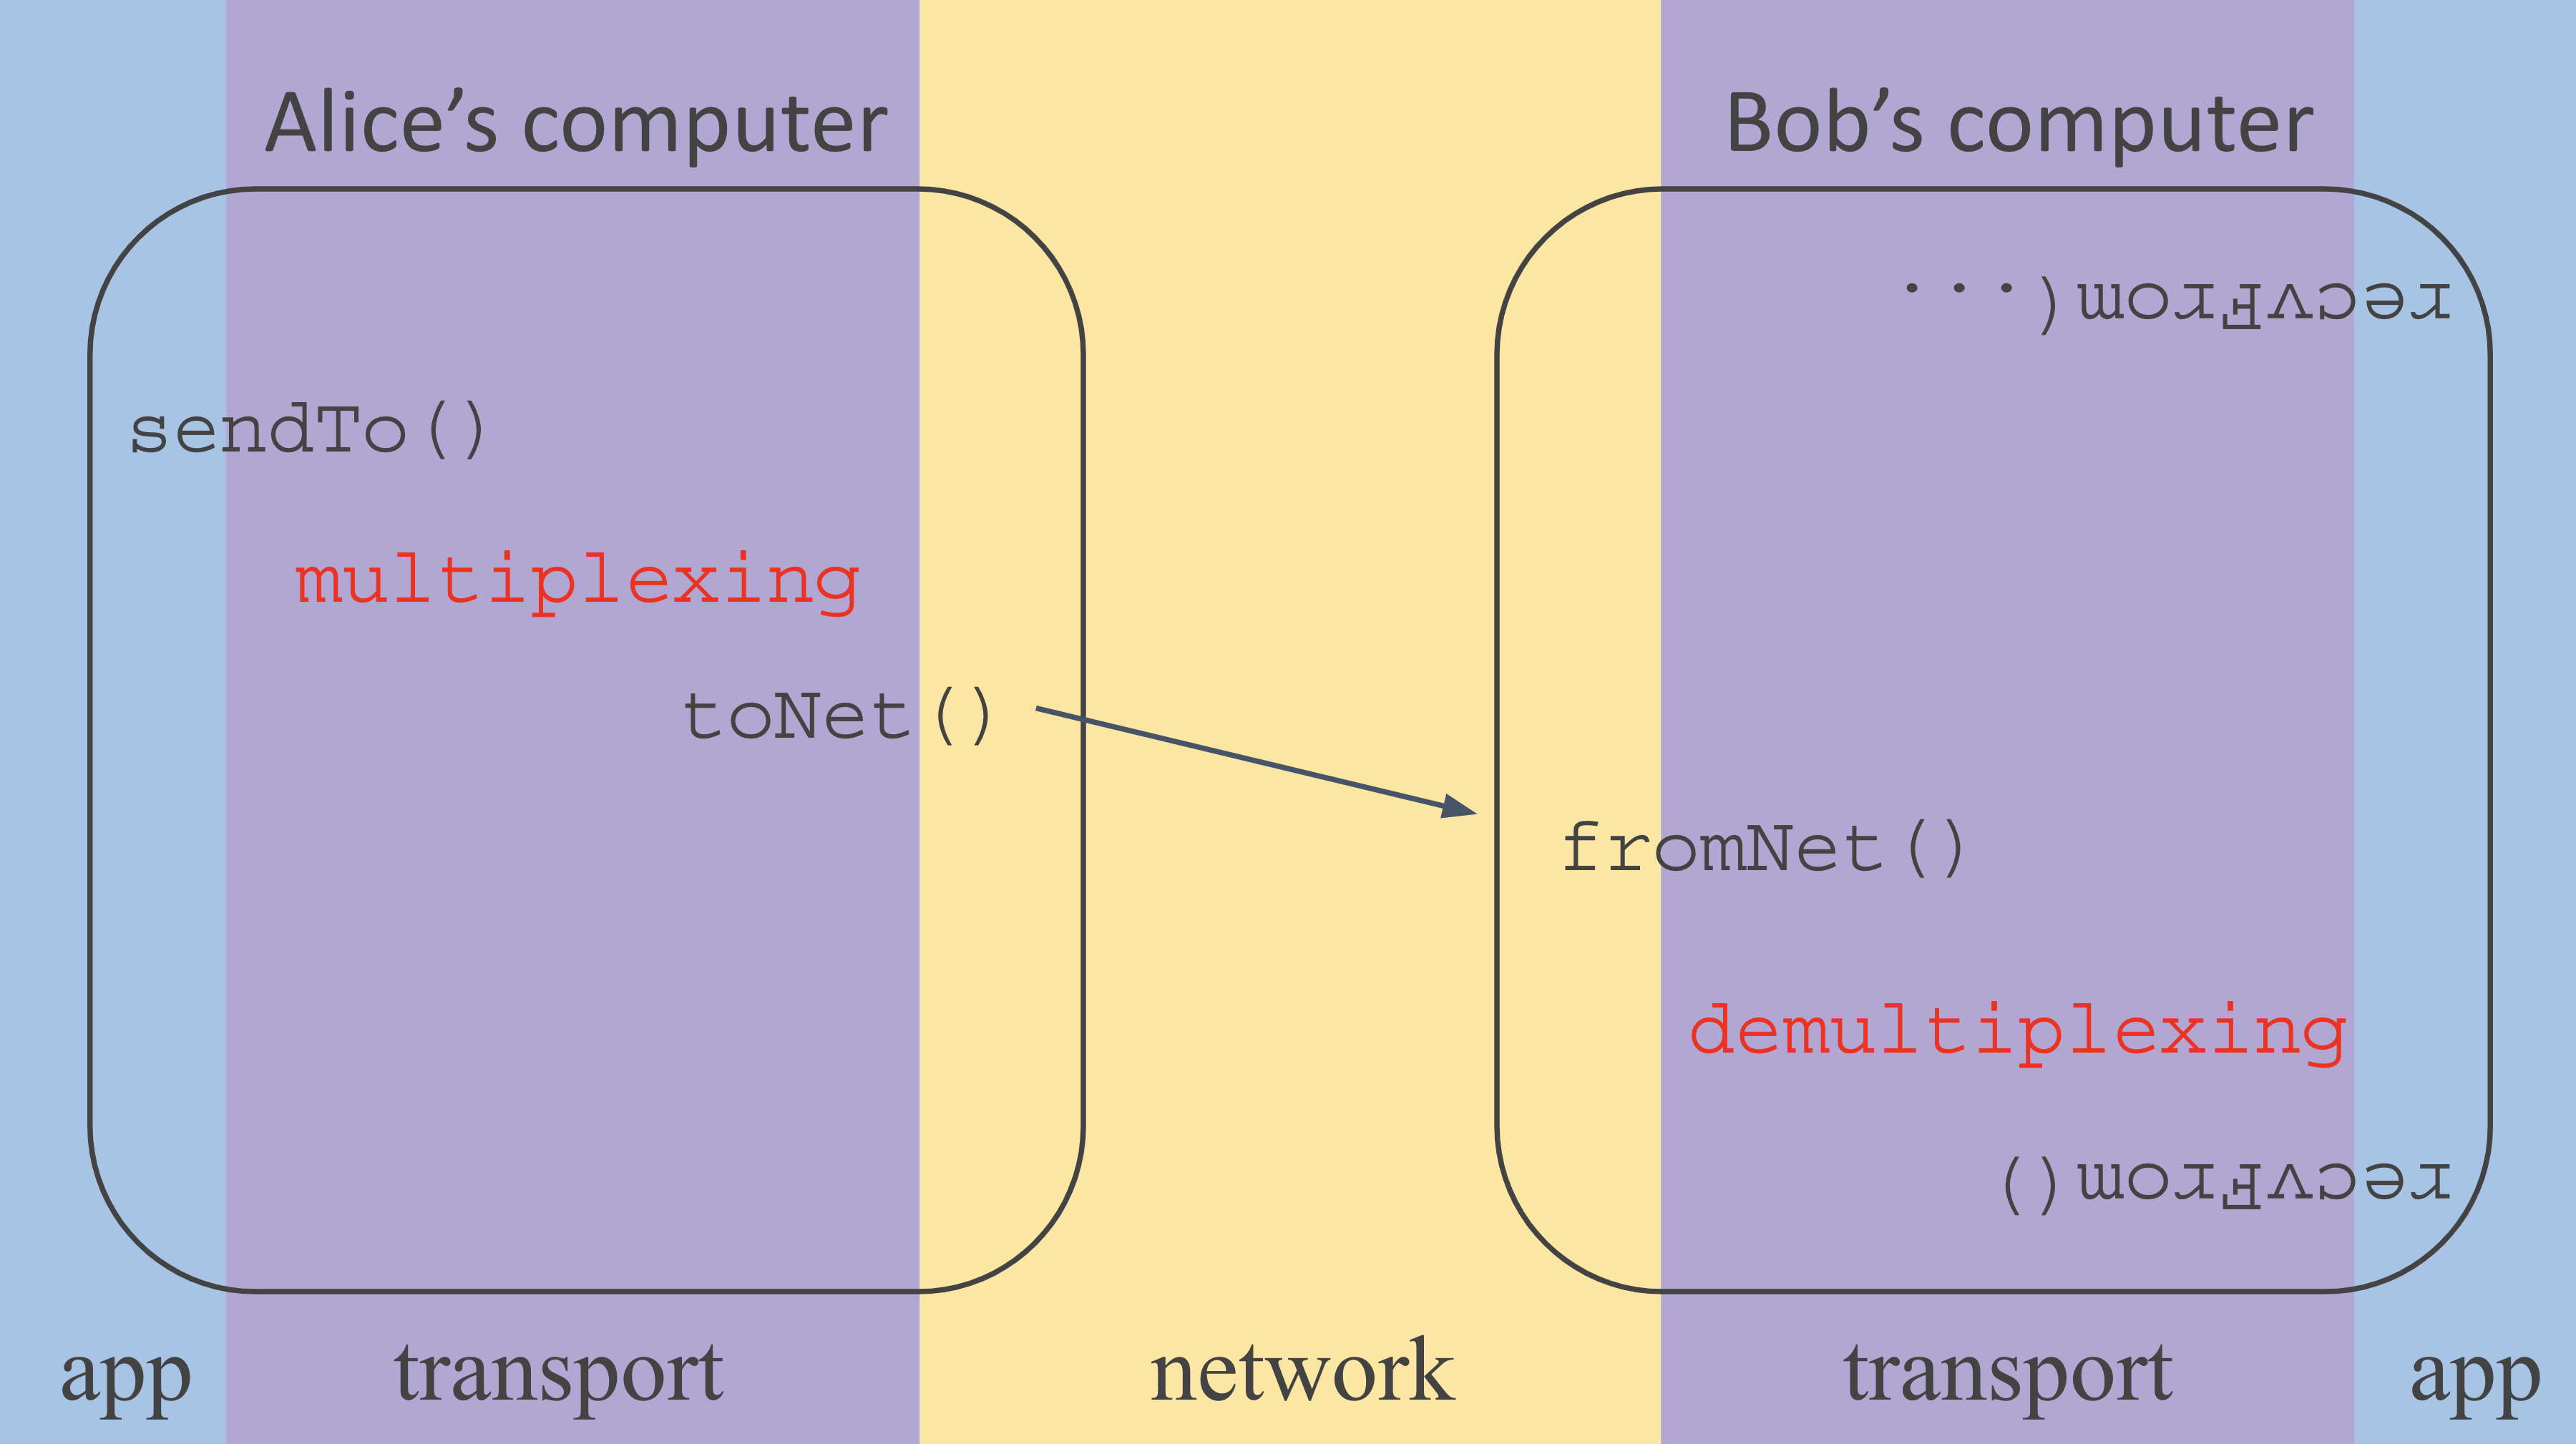
\includegraphics[width=0.5\textwidth]{images/udp.png}
\end{center}

\begin{enumerate}
  \item Both processes create UDP sockets: \texttt{socket()}
  \item Server binds to specific address: \texttt{bind()}
  \item Server prepares to receive: \texttt{recvfrom()}
  \item Client sends message: \texttt{sendto()}
  \item Transport layers handle UDP datagram transmission
  \item Server receives message and \texttt{recvfrom()} returns
\end{enumerate}

\subsection{UDP Header Structure and Limitations}
\textit{Understanding UDP's simple structure and constraints.}

\subsubsection{UDP Header (8 bytes total)}
\begin{itemize}
  \item[-] \textbf{Source Port (16 bits)} — Sending process identifier
  \item[-] \textbf{Destination Port (16 bits)} — Receiving process identifier  
  \item[-] \textbf{Length (16 bits)} — Total datagram length
  \item[-] \textbf{Checksum (16 bits)} — Error detection value
\end{itemize}

\subsubsection{UDP Capabilities and Limitations}
\begin{itemize}
  \item[-] \textbf{Provides:} Process identification, basic error detection, low overhead
  \item[-] \textbf{Lacks:} Reliability guarantees, ordering, flow control, congestion control, error correction
\end{itemize}

The network layer operates on a \textbf{best-effort} basis, potentially dropping, corrupting, or reordering packets. UDP provides a minimal abstraction over this unreliable foundation.

\section{Transmission Control Protocol (TCP)}
\textit{A comprehensive transport protocol providing reliable, ordered data delivery.}

TCP builds upon UDP's basic services while adding connection management, reliability, flow control, and congestion control.

\subsection{TCP Connection Management}
\textit{How TCP establishes and maintains reliable communication channels.}

\subsubsection{Connection Establishment: Three-Way Handshake}
Unlike UDP's connectionless approach, TCP requires establishing a logical connection before data exchange. This ensures both parties are ready to communicate and agree on communication parameters.

\begin{center}
  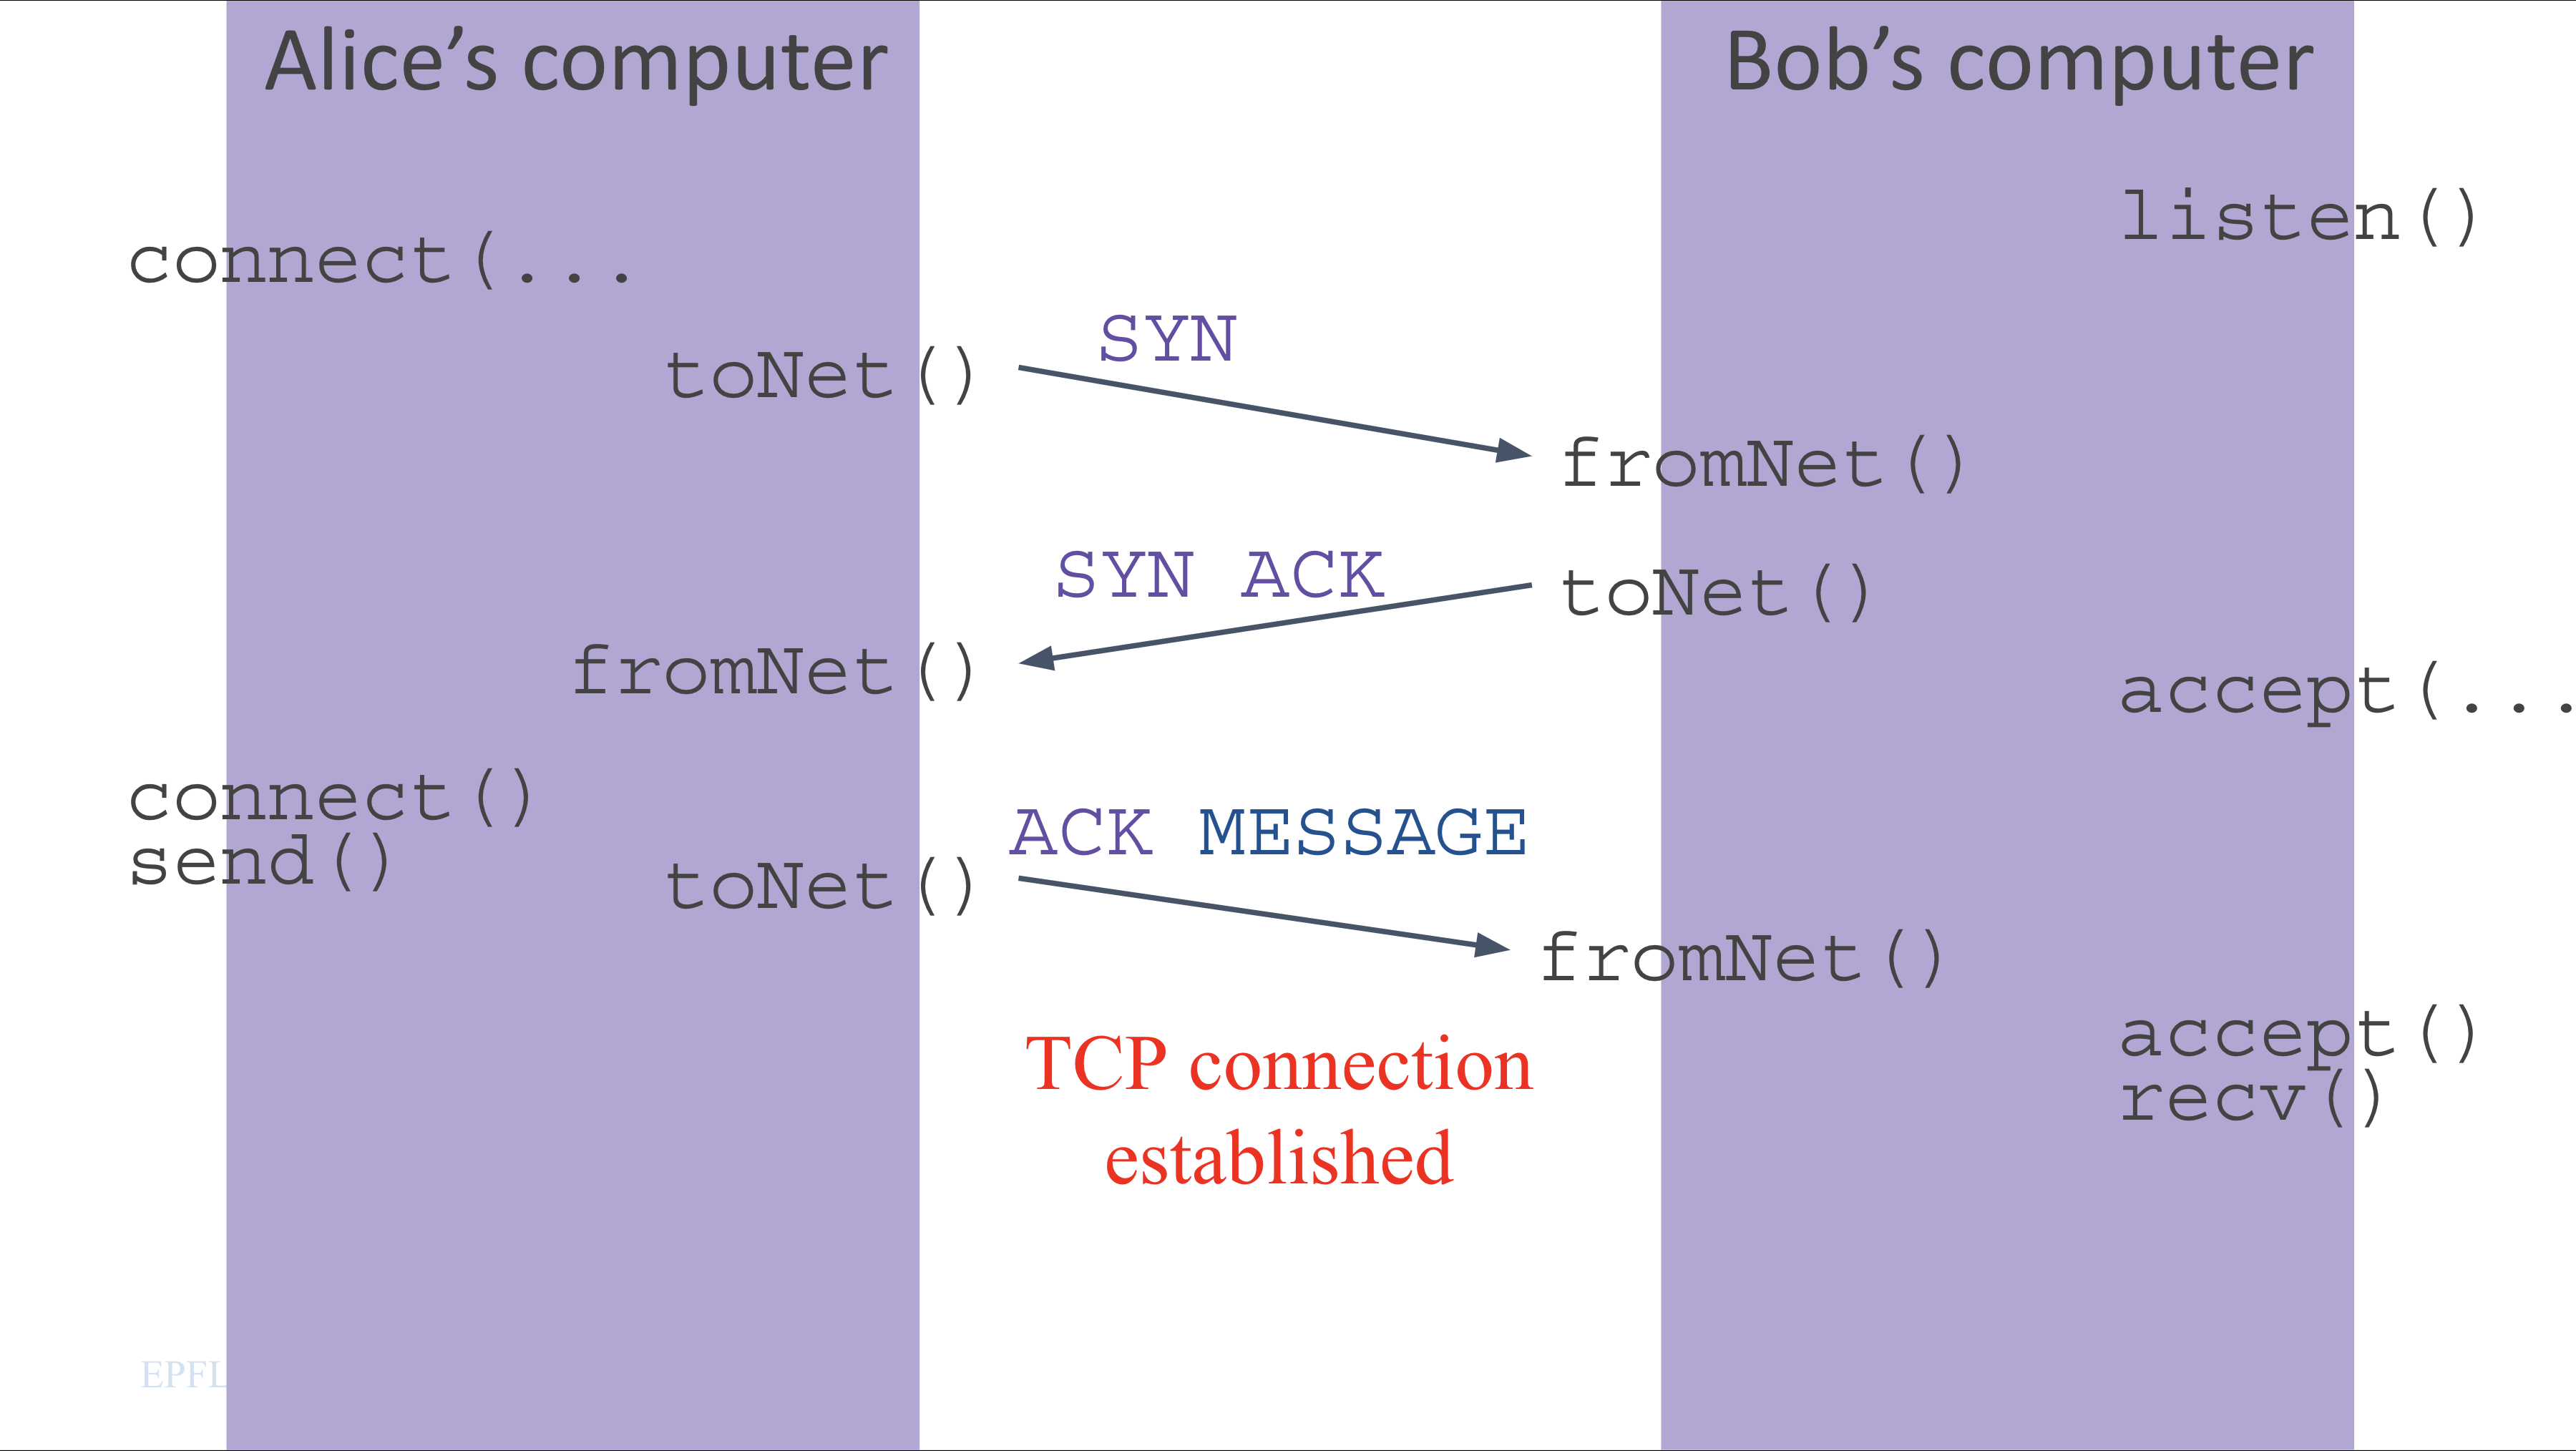
\includegraphics[width=0.5\textwidth]{images/handshake.png}
\end{center}

\paragraph{Handshake Concept.} The connection establishment works like a conversation:
\begin{enumerate}
  \item \textbf{Client Request:} "I want to establish a connection with you"
  \item \textbf{Server Response:} "I accept your request, and I also want to establish a connection with you"
  \item \textbf{Client Confirmation:} "I acknowledge your acceptance, connection established"
\end{enumerate}

\paragraph{Technical Implementation.} TCP implements this using control flags in segment headers:

\begin{enumerate}
  \item \textbf{Server Setup:} \texttt{socket()}, \texttt{bind()}, \texttt{listen()}
  \item \textbf{Client Initiation:} \texttt{socket()}, \texttt{connect()} → sends \textbf{SYN} (synchronize) segment
  \item \textbf{Server Response:} Sends \textbf{SYN-ACK} (synchronize-acknowledge) segment
  \item \textbf{Client Confirmation:} Sends \textbf{ACK} (acknowledge) segment (may include data)
  \item \textbf{Server Acceptance:} \texttt{accept()} creates connection socket
\end{enumerate}

\paragraph{Resource Allocation.} During handshake, both sides allocate send/receive buffers and establish connection state (sequence numbers, window sizes).

\subsection{TCP Socket Types and Multiplexing}
\textit{Understanding TCP's sophisticated connection management.}

\subsubsection{Socket Type Distinction}
\begin{itemize}
  \item[-] \textbf{Listening Socket} — Server uses for accepting new connections (\texttt{socket()}, \texttt{bind()}, \texttt{listen()})
  \item[-] \textbf{Connection Socket} — Dedicated to specific client-server communication, created by \texttt{accept()}
  \item[-] \textbf{Connection Identification} — Four-tuple: (source IP, source port, destination IP, destination port)
\end{itemize}

\subsubsection{Key Differences from UDP}
\begin{itemize}
  \item[-] Each TCP connection socket communicates with exactly one remote process
  \item[-] Servers can handle multiple simultaneous connections using separate connection sockets
  \item[-] Client uses \texttt{connect()} to establish connection to specific server process
  \item[-] Server uses \texttt{accept()} to create dedicated socket for each client connection
\end{itemize}

\subsection{TCP Reliability Mechanisms}
\textit{How TCP ensures reliable data delivery over unreliable networks.}

TCP implements comprehensive reliability mechanisms to overcome network limitations including corruption, loss, and reordering.

\subsubsection{Error Detection and Acknowledgment}
\textbf{Basic Operation:}
\begin{enumerate}
  \item Sender transmits TCP segment with data and sequence number
  \item Receiver verifies integrity using checksum
  \item If uncorrupted: receiver sends ACK and delivers data to application
  \item If corrupted or lost: sender detects via timeout and retransmits
\end{enumerate}

\subsubsection{Sequence Numbers and Acknowledgments}
\textbf{Sequence Numbers:}
\begin{itemize}
  \item[-] Identify data bytes: sequence number indicates the first data byte in segment
  \item[-] Enable duplicate detection: retransmitted segments have same sequence number
  \item[-] Support ordered delivery: receiver can reorder segments if needed
\end{itemize}

\textbf{Cumulative Acknowledgments:}
\begin{itemize}
  \item[-] ACK $n$ means "I have received all bytes up to and including byte $n-1$, expecting byte $n$"
  \item[-] No explicit negative ACKs: repeated ACKs serve as implicit NACKs
  \item[-] Simplifies protocol: single ACK field confirms multiple segments
\end{itemize}

\paragraph{Example.} If sender transmits SEQ 1 then SEQ 2, and receiver responds with ACK 2 twice, the second ACK 2 implicitly signals that SEQ 2 was not received correctly.

\subsubsection{Timeout and Retransmission}
\textbf{Timeout Mechanism:}
\begin{itemize}
  \item[-] Sender starts timer for each transmitted segment
  \item[-] If ACK not received before timeout, assume segment lost and retransmit
  \item[-] Handles both segment loss and ACK loss scenarios
  \item[-] May cause unnecessary retransmissions due to delayed ACKs
\end{itemize}

\textbf{Timeout Calculation:}
\begin{align}
\text{EstimatedRTT} &= 0.875 \times \text{EstimatedRTT} + 0.125 \times \text{SampleRTT} \\
\text{Timeout} &= \text{EstimatedRTT} + 4 \times \text{DevRTT}
\end{align}

Where DevRTT measures RTT variance. Conservative estimation prevents premature timeouts while adapting to network conditions.

\subsection{TCP Header Structure}
\textit{Understanding the complexity required for reliable communication.}

\subsubsection{Key TCP Header Fields (minimum 20 bytes)}
\begin{itemize}
  \item[-] \textbf{Source/Destination Ports} — Process identification
  \item[-] \textbf{Sequence Number} — First data byte number in this segment
  \item[-] \textbf{Acknowledgment Number} — Next expected byte number
  \item[-] \textbf{Control Flags} — SYN, ACK, FIN, RST for connection management
  \item[-] \textbf{Window Size} — Flow control information
  \item[-] \textbf{Checksum} — Error detection
\end{itemize}

\subsubsection{Control Flags}
\begin{itemize}
  \item[-] \textbf{SYN} — Connection establishment (handshake), 1-bit field
  \item[-] \textbf{ACK} — Acknowledgment field is valid
  \item[-] \textbf{FIN} — Connection termination
  \item[-] \textbf{RST} — Immediate connection reset
\end{itemize}

\section{Reliability Mechanisms Summary}
\textit{Comprehensive overview of transport layer reliability techniques.}

\subsection{Basic Reliability Components}
TCP achieves reliable data delivery through the combination of three fundamental mechanisms:

\begin{enumerate}
  \item \textbf{Checksums} — Detect corruption in transmitted data
  \item \textbf{Sequence Numbers + Acknowledgments + Retransmissions} — Overcome corruption through confirmed delivery
  \item \textbf{Timeouts + Sequence Numbers + Acknowledgments + Retransmissions} — Detect and overcome loss
\end{enumerate}

\subsection{Protocol Comparison}
\textit{Understanding when to use UDP vs TCP.}

\subsubsection{Protocol Trade-offs}
\begin{itemize}
  \item[-] \textbf{UDP:} Low overhead (8-byte header), fast, simple; no reliability guarantees
  \item[-] \textbf{TCP:} Higher overhead ($\geq$20-byte header), complex; provides reliability, ordering, flow control
\end{itemize}

\subsubsection{Application Suitability}
\begin{itemize}
  \item[-] \textbf{UDP Applications:} Real-time communication (VoIP, gaming), DNS queries, streaming media
  \item[-] \textbf{TCP Applications:} File transfer (HTTP, FTP), email, remote login (SSH), e-commerce
\end{itemize}

\paragraph{Design Principle.} The transport layer demonstrates a fundamental trade-off in protocol design: simplicity and efficiency versus feature richness and guarantees. Both approaches serve different application requirements in the Internet ecosystem.

\section{TCP Bidirectional Communication}
\textit{Understanding sequence numbers and acknowledgments in realistic scenarios.}

In practice, TCP connections carry bidirectional communication where both client and server processes exchange data simultaneously. This requires careful coordination of sequence numbers and acknowledgments.

\subsection{Bidirectional Data Exchange}
\textit{How TCP handles simultaneous data transmission in both directions.}

\subsubsection{Basic Bidirectional Example}
Consider a simple exchange where both client and server send single-byte messages:

\begin{itemize}
  \item[-] \textbf{Client sends "A":} SEQ 1, ACK 1 (first byte to server, expecting server's first byte)
  \item[-] \textbf{Server sends "B":} SEQ 1, ACK 2 (first byte to client, received client's byte 1, expecting byte 2)
\end{itemize}

\paragraph{Key Insight.} Each TCP segment contains both data (if any) and acknowledgment information, enabling efficient bidirectional communication without separate ACK-only segments.

\subsubsection{Multi-Byte Message Example}
\textit{Realistic example with variable-length messages.}

Consider an application-layer exchange:
\begin{itemize}
  \item[-] Client sends: "hello" (5 bytes)
  \item[-] Server responds: "hey" (3 bytes)  
  \item[-] Client responds: "all ok" (6 bytes)
  \item[-] Server responds: "bye" (3 bytes)
\end{itemize}

\begin{center}
  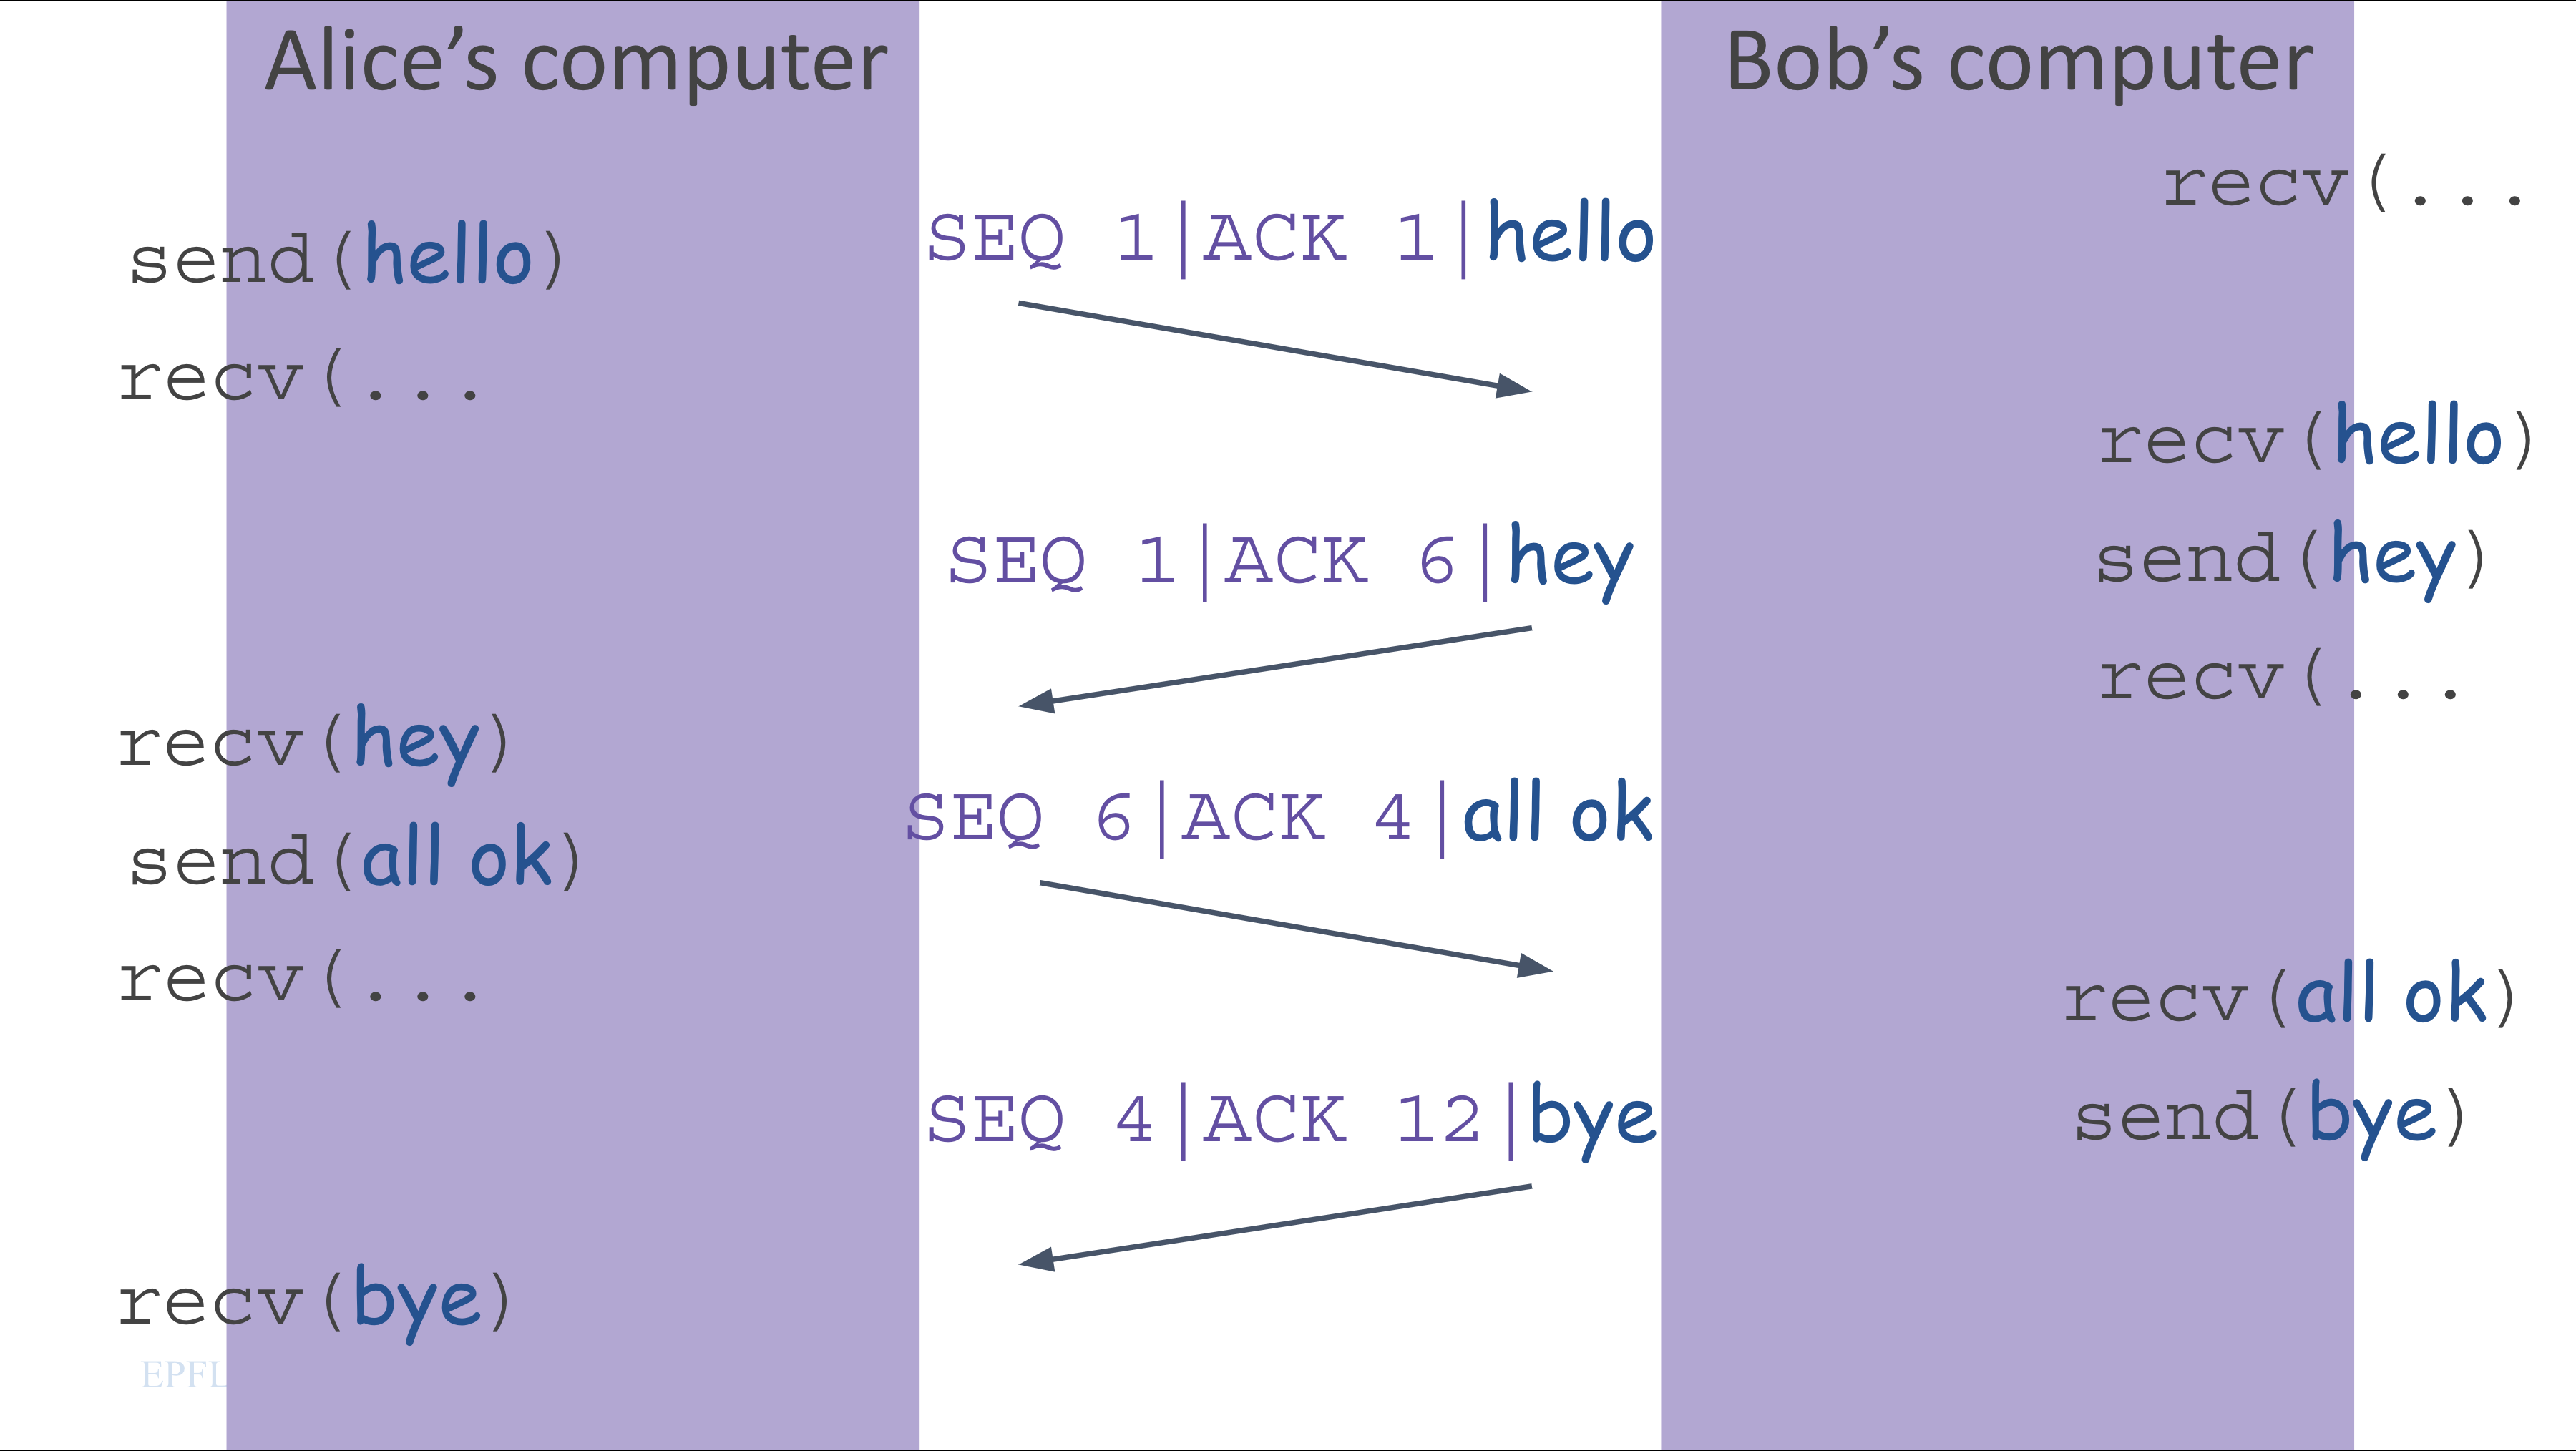
\includegraphics[width=0.5\textwidth]{images/alice-bob.png}
\end{center}

\textbf{Transport Layer Implementation:}
\begin{enumerate}
  \item \textbf{Client → Server:} "hello" with SEQ 1, ACK 1
  \item \textbf{Server → Client:} "hey" with SEQ 1, ACK 6 (received bytes 1-5, expecting byte 6)
  \item \textbf{Client → Server:} "all ok" with SEQ 6, ACK 4 (received bytes 1-3, expecting byte 4)
  \item \textbf{Server → Client:} "bye" with SEQ 4, ACK 12 (received bytes 6-11, expecting byte 12)
\end{enumerate}

\subsection{Real-World HTTP Example}
\textit{Analyzing TCP behavior in web communication.}

\subsubsection{HTTP Request-Response Pattern}
Web communication demonstrates practical TCP usage with asymmetric data flows:

\begin{itemize}
  \item[-] \textbf{Client:} HTTP GET request (200 bytes)
  \item[-] \textbf{Server:} HTTP response with data (3,100 bytes)
\end{itemize}

\subsubsection{Segmentation and Acknowledgment Pattern}
\textbf{Client Request:}
\begin{itemize}
  \item[-] Single segment: SEQ 1, ACK 1 (200-byte GET request)
\end{itemize}

\textbf{Server Response (segmented):}
\begin{itemize}
  \item[-] Segment 1: SEQ 1, ACK 201 (bytes 1-1500)
  \item[-] Segment 2: SEQ 1501, ACK 201 (bytes 1501-3000)  
  \item[-] Segment 3: SEQ 3001, ACK 201 (bytes 3001-3100)
\end{itemize}

\textbf{Client Acknowledgments:}
\begin{itemize}
  \item[-] ACK 1501: Confirming receipt of first 1500 server bytes
  \item[-] ACK 3001: Confirming receipt of bytes 1-3000
  \item[-] ACK 3101: Confirming receipt of entire response
\end{itemize}

\subsubsection{Important Observations}
\begin{itemize}
  \item[-] \textbf{Persistent SEQ:} Client ACKs use SEQ 201 (no new data to send)
  \item[-] \textbf{Cumulative ACKs:} Each ACK confirms all bytes received so far
  \item[-] \textbf{Data Segmentation:} Large messages split across multiple segments for efficient transmission
  \item[-] \textbf{Piggybacked ACKs:} Acknowledgments combined with data when possible
\end{itemize}

\paragraph{Segmentation Rationale.} Transport layers segment large messages to optimize network utilization and enable efficient error recovery at the segment level rather than requiring retransmission of entire large messages.

\section{TCP Flow Control and Congestion Control}
\textit{Managing sender transmission rates to prevent receiver overload and network congestion.}

TCP must control the rate at which data is transmitted to prevent overwhelming both the receiver and the network infrastructure. This requires two complementary mechanisms operating simultaneously.

\subsection{Maximum Segment Size and Segmentation}
\textit{Understanding how TCP determines segment boundaries.}

\subsubsection{Maximum Segment Size (MSS)}
The Maximum Segment Size represents the maximum amount of application-layer data that a single TCP segment may carry:

\begin{itemize}
  \item[-] \textbf{Determination:} MSS is dictated by network properties, particularly the bit error rate of links between sender and receiver
  \item[-] \textbf{Discovery:} Transport layer discovers MSS through network interface properties and path MTU discovery
  \item[-] \textbf{Typical Value:} 1500 bytes in current Internet infrastructure
  \item[-] \textbf{Impact:} Large messages require segmentation across multiple TCP segments
\end{itemize}

\subsubsection{Practical Segmentation Example}
Consider an HTTP response scenario:
\begin{itemize}
  \item[-] Client sends 200-byte GET request → Single segment
  \item[-] Server responds with 3100-byte data → Three segments (1500 + 1500 + 100 bytes)
  \item[-] Each segment acknowledged independently for reliable delivery
\end{itemize}

\subsection{Sender Window Management}
\textit{Controlling the maximum number of unacknowledged bytes in transmission.}

\subsubsection{Sender Window Concept}
The \textbf{sender window} indicates the maximum number of unacknowledged bytes that the sender may transmit:

\begin{itemize}
  \item[-] \textbf{Purpose:} Prevents overwhelming receiver and network
  \item[-] \textbf{Dynamic Adjustment:} Changes based on current network and receiver conditions
  \item[-] \textbf{Computation:} Minimum of flow control window and congestion control window
\end{itemize}

\subsubsection{Dual Control Mechanisms}
TCP sender window management combines two independent mechanisms:

\begin{enumerate}
  \item \textbf{Flow Control} — Prevents overwhelming the receiver
  \begin{itemize}
    \item[-] Receiver explicitly signals maximum acceptable unacknowledged bytes
    \item[-] Communicated via receiver window field in TCP header
    \item[-] Direct feedback mechanism
  \end{itemize}

  \item \textbf{Congestion Control} — Prevents overwhelming the network
  \begin{itemize}
    \item[-] Sender estimates network capacity independently
    \item[-] No explicit network feedback available
    \item[-] Inferred through packet loss and acknowledgment patterns
  \end{itemize}
\end{enumerate}

\textbf{Window Computation.} \\
At each moment: $\text{Sender Window} = \min(\text{Flow Control Window}, \text{Congestion Window})$
\newpage
\section{TCP Congestion Control Algorithms}
\textit{Adaptive algorithms for inferring and responding to network congestion.}

TCP congestion control operates on the principle of \textbf{self-clocking}, where the sender adjusts its transmission rate based on acknowledgment patterns without explicit network feedback.

\subsection{Key Congestion Control Concepts}
\textit{Essential terminology and variables for understanding TCP algorithms.}

\subsubsection{Slow Start Threshold (ssthresh)}
The \textbf{slow start threshold} is a critical variable that acts as TCP's "memory" of previous network congestion:

\begin{itemize}
  \item[-] \textbf{Purpose:} Remembers the congestion window size when congestion was last detected
  \item[-] \textbf{Initial Value:} Set to a large value (effectively infinite) when connection starts
  \item[-] \textbf{Updated When:} Congestion occurs (timeout or duplicate acknowledgments)
  \item[-] \textbf{Calculation:} Always set to half the current congestion window when congestion detected
  \item[-] \textbf{Usage:} Determines when to switch from exponential growth to linear growth
\end{itemize}

\paragraph{Why Half the Window?} When congestion occurs, TCP assumes the network can handle approximately half of what was being sent, providing a conservative estimate for future transmissions.

\subsubsection{Congestion Window (cwnd)}
The \textbf{congestion window} represents the sender's estimate of how much data the network can handle:

\begin{itemize}
  \item[-] \textbf{Purpose:} Controls the maximum unacknowledged data the sender may transmit
  \item[-] \textbf{Initial Value:} 1 Maximum Segment Size (conservative start)
  \item[-] \textbf{Dynamic Adjustment:} Increases when network performs well, decreases when congestion detected
  \item[-] \textbf{Units:} Measured in bytes
\end{itemize}

\subsubsection{Maximum Segment Size}
The \textbf{Maximum Segment Size} is the largest amount of application data that fits in one TCP segment:

\begin{itemize}
  \item[-] \textbf{Typical Value:} 1500 bytes in most modern networks
  \item[-] \textbf{Determined By:} Network path properties and interface capabilities
  \item[-] \textbf{Usage:} Unit of measurement for window adjustments
\end{itemize}

\subsection{Self-Clocking Principle}
\textit{How TCP infers network conditions from acknowledgment behavior.}

\subsubsection{Basic Self-Clocking Logic}
The sender makes decisions based on acknowledgment patterns, following this simple logic:

\begin{itemize}
  \item[-] \textbf{New acknowledgment received} → Network conditions good → Increase congestion window
  \item[-] \textbf{No new acknowledgment (timeout)} → Network conditions bad → Decrease congestion window
  \item[-] \textbf{Adaptive Behavior} → Continuously adjusts to changing network conditions
\end{itemize}

\paragraph{Step-by-Step Decision Process:}
\begin{enumerate}
  \item Send data segments up to the current congestion window limit
  \item Wait for acknowledgments from the receiver
  \item \textbf{If acknowledgments arrive promptly:} Network can handle current load → increase window size
  \item \textbf{If acknowledgments are missing or delayed:} Network may be congested → decrease window size
  \item Repeat this process for every round of transmission
\end{enumerate}

\subsubsection{Algorithm Variations}
Multiple congestion control algorithms implement this principle with different strategies:
\begin{itemize}
  \item[-] \textbf{Historical Algorithms:} Tahoe and Reno (foundational concepts we will study)
  \item[-] \textbf{Modern Algorithms:} Cubic, New Reno (currently deployed in practice)
  \item[-] \textbf{Key Design Questions:} How aggressively to react to new acknowledgments vs. missing acknowledgments
\end{itemize}

\subsection{TCP Tahoe Algorithm}
\textit{Foundational congestion control algorithm demonstrating core principles.}

The Tahoe algorithm operates in two distinct states, each with different strategies for growing the congestion window based on network feedback.

\subsubsection{Tahoe Algorithm States}

\paragraph{Slow Start State.} Aggressive window growth for initial connection:
\begin{itemize}
  \item[-] \textbf{Initial Window:} 1 Maximum Segment Size (conservative start)
  \item[-] \textbf{Growth Rule:} Increase window by 1 Maximum Segment Size for each new acknowledgment received
  \item[-] \textbf{Growth Pattern:} Window doubles every round-trip time (exponential growth)
  \item[-] \textbf{Transition Condition:} Switch to congestion avoidance when window reaches slow start threshold
\end{itemize}

\paragraph{Slow Start Step-by-Step Process:}
\begin{enumerate}
  \item Start with congestion window = 1 Maximum Segment Size
  \item Send data segments up to the current window limit
  \item For each acknowledgment received, increase window by 1 Maximum Segment Size
  \item Send more data with the larger window
  \item Continue until window size equals slow start threshold
\end{enumerate}

\paragraph{Congestion Avoidance State.} Cautious window growth near suspected limits:
\begin{itemize}
  \item[-] \textbf{Growth Rule:} Increase window by $\frac{\text{Maximum Segment Size}^2}{\text{current window size}}$ for each new acknowledgment
  \item[-] \textbf{Growth Pattern:} Window increases by approximately 1 Maximum Segment Size per round-trip time (linear growth)
  \item[-] \textbf{Purpose:} Probe for additional network capacity carefully without causing congestion
\end{itemize}

\paragraph{Congestion Avoidance Step-by-Step Process:}
\begin{enumerate}
  \item Current window size has reached slow start threshold
  \item Send data segments up to the current window limit
  \item For each acknowledgment received, increase window by $\frac{\text{Maximum Segment Size}^2}{\text{current window size}}$ bytes
  \item This small increase results in approximately 1 Maximum Segment Size growth per round-trip time
  \item Continue until congestion is detected (timeout occurs)
\end{enumerate}

\subsubsection{Tahoe Transition Events}

\paragraph{Timeout Event.} Response to suspected severe congestion:

When the sender waits too long for an acknowledgment (timeout occurs), it assumes severe network congestion and responds conservatively:

\begin{enumerate}
  \item \textbf{Update slow start threshold:} Set slow start threshold = $\frac{\text{current window size}}{2}$ (remember where congestion occurred)
  \item \textbf{Reset congestion window:} Set congestion window back to 1 Maximum Segment Size (start over conservatively)
  \item \textbf{Retransmit lost data:} Send the oldest unacknowledged segment again
  \item \textbf{Return to slow start state:} Begin exponential growth again, but more cautiously
\end{enumerate}

\paragraph{Why These Steps?}
\begin{itemize}
  \item[-] \textbf{Halving the threshold:} Assumes network can handle about half of what caused congestion
  \item[-] \textbf{Resetting to 1:} Conservative restart ensures we don't immediately cause more congestion
  \item[-] \textbf{Retransmission:} Ensures data reliability despite network problems
  \item[-] \textbf{Slow start restart:} Allows gradual ramp-up to test current network conditions
\end{itemize}

\paragraph{Window Reaches Slow Start Threshold.} Transition to careful growth:

When the congestion window grows to equal the slow start threshold during slow start:

\begin{enumerate}
  \item \textbf{State change:} Switch from slow start to congestion avoidance
  \item \textbf{Window maintenance:} Keep current window size unchanged
  \item \textbf{Growth pattern change:} Begin linear growth instead of exponential growth
  \item \textbf{Rationale:} We're approaching the size that previously caused congestion, so be more careful
\end{enumerate}

\subsection{Detailed Tahoe Example}
\textit{Step-by-step illustration of Tahoe algorithm behavior.}

\subsubsection{Scenario Setup}
Consider Alice establishing a TCP connection to Bob with Maximum Segment Size = 100 bytes:

\begin{itemize}
  \item[-] \textbf{Connection Established:} Three-way handshake completed successfully
  \item[-] \textbf{Initial State:} Alice starts in slow start state
  \item[-] \textbf{Initial Congestion Window:} 1 Maximum Segment Size = 100 bytes
  \item[-] \textbf{Initial Slow Start Threshold:} Undefined (will be set after first congestion event)
\end{itemize}

\paragraph{What Alice Will Do:}
Alice will start sending data conservatively, then gradually increase her sending rate based on network feedback. Let's trace through exactly what happens step by step.

\subsubsection{Phase 1: Slow Start Growth}

\paragraph{Round 1 — Conservative Beginning:}
\begin{itemize}
  \item[-] \textbf{Alice sends:} Sequence 1 (bytes 1-100), current window = 100 bytes
  \item[-] \textbf{Bob responds:} Acknowledgment 101 (confirming receipt of bytes 1-100)
  \item[-] \textbf{Window update:} Alice increases window: 100 + 100 = 200 bytes (doubled)
  \item[-] \textbf{Explanation:} Alice received 1 acknowledgment, so she adds 1 Maximum Segment Size to her window
\end{itemize}

\paragraph{Round 2 — Exponential Growth:}
\begin{itemize}
  \item[-] \textbf{Alice sends:} Sequence 101 (bytes 101-200), Sequence 201 (bytes 201-300)
  \item[-] \textbf{Bob responds:} Acknowledgment 201, Acknowledgment 301
  \item[-] \textbf{Window update:} Alice increases window: 200 + 100 + 100 = 400 bytes (doubled again)
  \item[-] \textbf{Explanation:} Alice received 2 acknowledgments, so she adds 2 Maximum Segment Sizes to her window
\end{itemize}

\paragraph{Round 3 — Network Limit Reached:}
\begin{itemize}
  \item[-] \textbf{Alice sends:} Sequence 301, Sequence 401, Sequence 501, Sequence 601 (400 bytes total)
  \item[-] \textbf{Network congestion:} All 4 segments lost due to network overload
  \item[-] \textbf{Timeout occurs:} Alice detects no acknowledgments received within timeout period
  \item[-] \textbf{Alice's conclusion:} The network cannot handle 400 bytes sent simultaneously
\end{itemize}

\subsubsection{Phase 2: Timeout Response and Recovery}

\paragraph{Congestion Detection and Response:}

Alice now realizes the network is congested and responds with the Tahoe algorithm's timeout procedure:

\begin{enumerate}
  \item \textbf{Set slow start threshold:} $\frac{400}{2} = 200$ bytes (remember where congestion occurred)
  \item \textbf{Reset congestion window:} 400 → 100 bytes (back to 1 Maximum Segment Size)
  \item \textbf{Return to slow start state:} Begin conservative exponential growth again
  \item \textbf{Retransmit lost data:} Send Sequence 301 (oldest unacknowledged segment)
\end{enumerate}

\paragraph{Why Alice Does This:}
\begin{itemize}
  \item[-] \textbf{Threshold = 200 bytes:} Alice remembers that 400 bytes caused problems, so 200 bytes is probably safe
  \item[-] \textbf{Window = 100 bytes:} Start conservatively to avoid immediately causing more congestion
  \item[-] \textbf{Slow start state:} Use exponential growth to quickly find the right sending rate
  \item[-] \textbf{Retransmit:} Ensure data reliability by resending what was lost
\end{itemize}

\paragraph{Recovery Transmission:}
\begin{itemize}
  \item[-] \textbf{Alice sends:} Sequence 301, current window = 100 bytes
  \item[-] \textbf{Bob responds:} Acknowledgment 401 (confirming receipt of bytes 301-400)
  \item[-] \textbf{Window update:} Alice increases window: 100 + 100 = 200 bytes
  \item[-] \textbf{Important:} Window now equals slow start threshold (200 bytes)
\end{itemize}

\subsubsection{Phase 3: Transition to Congestion Avoidance}

\paragraph{Reaching Slow Start Threshold:}
\begin{itemize}
  \item[-] \textbf{Current window:} 200 bytes = slow start threshold
  \item[-] \textbf{State change:} Slow start → Congestion avoidance
  \item[-] \textbf{Alice sends:} Sequence 401, Sequence 501 (200 bytes total)
  \item[-] \textbf{Reason for change:} Alice is approaching the window size that previously caused congestion
\end{itemize}

\paragraph{Linear Growth Phase:}

Now Alice switches to much more conservative growth to avoid causing congestion again:

\begin{itemize}
  \item[-] \textbf{Acknowledgment 501 received:} Window = 200 + $\frac{100^2}{200}$ = 200 + 50 = 250 bytes
  \item[-] \textbf{Acknowledgment 601 received:} Window = 250 + $\frac{100^2}{250}$ = 250 + 40 = 290 bytes
  \item[-] \textbf{Acknowledgment 701 received:} Window = 290 + $\frac{100^2}{290}$ = 290 + 34 = 324 bytes
\end{itemize}

\paragraph{Understanding the Linear Growth Formula:}
\begin{itemize}
  \item[-] \textbf{Formula:} New window = Current window + $\frac{(\text{Maximum Segment Size})^2}{\text{Current window}}$
  \item[-] \textbf{Effect:} As window gets larger, the increase gets smaller per acknowledgment
  \item[-] \textbf{Result:} Window grows by approximately 1 Maximum Segment Size per round-trip time
  \item[-] \textbf{Contrast:} Much slower than slow start's exponential doubling
\end{itemize}

\newpage
\subsection{TCP Reno Algorithm Enhancement}
\textit{Improved congestion control with fast retransmit and fast recovery.}

TCP Reno enhances Tahoe by reacting more intelligently to packet loss, distinguishing between single segment loss and severe network congestion.

\subsubsection{Fast Retransmit Mechanism}

\paragraph{Duplicate ACK Detection Scenario:}
Consider Alice with 500-byte congestion window sending 5 segments where only the first is lost:

\begin{itemize}
  \item[-] \textbf{Alice sends:} SEQ 301, SEQ 401, SEQ 501, SEQ 601, SEQ 701
  \item[-] \textbf{Network behavior:} First segment (SEQ 301) lost, others received successfully
  \item[-] \textbf{Bob's response:} ACK 301, ACK 301, ACK 301, ACK 301 (duplicate ACKs)
\end{itemize}

\paragraph{Fast Retransmit Logic:}
Upon receiving 3 duplicate ACKs, Alice infers single segment loss rather than network collapse:
\begin{enumerate}
  \item \textbf{Immediate retransmit:} Send SEQ 301 without waiting for timeout
  \item \textbf{Set ssthresh:} $\frac{500}{2} = 250$ bytes
  \item \textbf{Enter fast recovery:} Specialized state for handling isolated loss
\end{enumerate}

\subsubsection{Fast Recovery State}

\paragraph{Window Inflation Strategy:}
Alice must handle segments that are officially unacknowledged but likely received:

\begin{enumerate}
  \item \textbf{Base window:} Set to ssthresh = 250 bytes
  \item \textbf{Inflation:} Add 3 MSS (300 bytes) for segments indicated by duplicate ACKs
  \item \textbf{Working window:} 250 + 300 = 550 bytes
  \item \textbf{New transmission:} Can send 50 additional bytes beyond already transmitted 500 bytes
\end{enumerate}

\paragraph{Continued Fast Recovery:}
For each additional duplicate ACK received:
\begin{itemize}
  \item[-] \textbf{Interpretation:} One more segment confirmed received by Bob
  \item[-] \textbf{Window adjustment:} Inflate by 1 MSS
  \item[-] \textbf{Transmission:} Send additional data if window permits
\end{itemize}

\paragraph{Recovery Completion:}
When Alice receives new ACK (e.g., ACK 801):
\begin{enumerate}
  \item \textbf{Conclusion:} Lost segment successfully retransmitted and received
  \item \textbf{State transition:} Exit fast recovery
  \item \textbf{Window reset:} Set congestion window to ssthresh (250 bytes)
  \item \textbf{Mode switch:} Enter congestion avoidance state
\end{enumerate}

\end{document}